%%
%% Copyright 2022 OXFORD UNIVERSITY PRESS
%%
%% This file is part of the 'oup-authoring-template Bundle'.
%% ---------------------------------------------
%%
%% It may be distributed under the conditions of the LaTeX Project Public
%% License, either version 1.2 of this license or (at your option) any
%% later version.  The latest version of this license is in
%%    http://www.latex-project.org/lppl.txt
%% and version 1.2 or later is part of all distributions of LaTeX
%% version 1999/12/01 or later.
%%
%% The list of all files belonging to the 'oup-authoring-template Bundle' is
%% given in the file `manifest.txt'.
%%
%% Template article for OXFORD UNIVERSITY PRESS's document class `oup-authoring-template'
%% with bibliographic references
%%

%%%CONTEMPORARY%%%
%\documentclass[unnumsec,webpdf,contemporary,large]{oup-authoring-template}%
%\documentclass[unnumsec,webpdf,contemporary,large,namedate]{oup-authoring-template}% uncomment this line for author year citations and comment the above
%\documentclass[unnumsec,webpdf,contemporary,medium]{oup-authoring-template}
%\documentclass[unnumsec,webpdf,contemporary,small]{oup-authoring-template}

%%%MODERN%%%
%\documentclass[unnumsec,webpdf,modern,large]{oup-authoring-template}
\documentclass[unnumsec,webpdf,modern,large,namedate]{oup-authoring-template}% uncomment this line for author year citations and comment the above
%\documentclass[unnumsec,webpdf,modern,medium]{oup-authoring-template}
%\documentclass[unnumsec,webpdf,modern,small]{oup-authoring-template}

%%%TRADITIONAL%%%
%\documentclass[unnumsec,webpdf,traditional,large]{oup-authoring-template}
%\documentclass[unnumsec,webpdf,traditional,large,namedate]{oup-authoring-template}% uncomment this line for author year citations and comment the above
%\documentclass[unnumsec,namedate,webpdf,traditional,medium]{oup-authoring-template}
%\documentclass[namedate,webpdf,traditional,small]{oup-authoring-template}

%\onecolumn % for one column layouts

%\usepackage{showframe}
\usepackage{fontenc}

\usepackage{graphicx}

% line numbers
% \usepackage[mathlines, switch]{lineno}
% \usepackage[right]{lineno}

\begin{document}

% \journaltitle{Bioinformatics}
\journaltitle{Preprint}
% \DOI{DOI HERE}
\copyrightyear{2023}
% \pubyear{2019}
% \access{Advance Access Publication Date: Day Month Year}
\appnotes{Paper}

\firstpage{1}

%\subtitle{Subject Section}

\title[tstrait]{tstrait: a quantitative trait simulator for ancestral recombination graphs}

\author[1,2,$\ast$]{Daiki Tagami\ORCID{0000-0002-0923-1070}}
\author[2]{Gertjan Bisschop\ORCID{0000-0001-8327-0142}}
\author[2]{Jerome Kelleher\ORCID{0000-0002-7894-5253}}

\authormark{D.Tagami et al.}

\address[1]{\orgdiv{Department of Statistics}, \orgname{University of Oxford},
\orgaddress{\street{24-29 St Giles'}, \postcode{Oxford OX1 3LB},
\country{United Kingdom}}}
\address[2]{\orgdiv{Big Data Institute,
Li Ka Shing Centre for Health Information and Discovery},
\orgname{University of Oxford}, \orgaddress{\street{Old Road Campus},
\postcode{Oxford OX3 7LF}, \country{United Kingdom}}}

\corresp[$\ast$]{Corresponding author.
\href{email:daiki.tagami@hertford.ox.ac.uk}{daiki.tagami@hertford.ox.ac.uk}}

\received{Date}{0}{Year}
\revised{Date}{0}{Year}
\accepted{Date}{0}{Year}

\abstract{
\textbf{Summary:}
Ancestral recombination graphs (ARGs) encode the ensemble of correlated
genealogical trees arising from recombination in a compact and efficient
structure, and are of fundamental importance in population and statistical
genetics. Recent breakthroughs have made it possible to simulate and
infer ARGs at biobank scale, and there is now intense interest
in using ARG-based methods across a broad range of applications,
particularly in genome-wide association studies (GWAS).
Sophisticated methods exist to simulate ARGs using
population genetics models, but there is currently no software
to simulate quantitative traits directly from these ARGs.
To apply existing quantitative trait simulators users must export
genotype data, losing important information about ancestral processes
and producing prohibitively large files when applied
to the biobank-scale datasets currently of interest in GWAS.
We present \texttt{tstrait},
an open-source Python library to simulate
quantitative traits on ARGs, and show how this user-friendly software
can quickly simulate phenotypes for biobank-scale datasets
on a laptop computer.
\\\textbf{Availability and Implementation:} \texttt{tstrait} is available
for download on the Python Package Index.
Full documentation with examples and workflow
templates is available on \url{https://tskit.dev/tstrait/docs/}, and the
development version is maintained on GitHub
(\url{https://github.com/tskit-dev/tstrait}).\\ \textbf{Contact:}
\href{daiki.tagami@hertford.ox.ac.uk}{daiki.tagami@hertford.ox.ac.uk}\\
}

%\abstract{Abstracts must be able to stand alone and so cannot contain %citations to
%the paper's references, equations, etc. An abstract must consist of a single
%paragraph and be concise. Because of online formatting, abstracts must appear
%as plain as possible.}
\keywords{Ancestral Recombination Graph, ARG, GWAS, quantitative traits,
simulation}

\maketitle

\section{Introduction}

Genome-wide association studies (GWAS)
identify genetic variants that are statistically
associated with a specific trait~\citep{uffelmann2021}.
Many loci that are associated with various human diseases and
traits have been
identified~\citep[e.g.][]{yengo2022,mathieson2023},
% \citep{locke2015,ishigaki2022,
% mahajan2022,yengo2022,mathieson2023},
and GWAS results are actively being incorporated into clinical
practice~\citep{visscher2017}.
The great success of GWAS has prompted the collection of many biobank
datasets consisting of hundreds of thousands of
participants~\citep{tanjo2021practical},
but this scale presents significant challenges to
current GWAS methodology~\citep{uffelmann2021}.

Simulation is a critical component of GWAS method development, and
generally consists of two steps:
first simulating genetic variation (genotypes)
and then simulating quantitative traits (phenotypes) based on the
synthetic genotypes.
The combined genotypes and phenotypes represent ground-truth data
which GWAS methods can be evaluated against.
Genetic variation is
usually simulated either by model-based population genetic
methods such as
\texttt{msprime}~\citep{baumdicker2022efficient}
and \texttt{SLiM}~\citep{haller2023},
or by statistical resampling from existing datasets
using methods like \texttt{HAPGEN2}~\citep{su2011hapgen2}
and \texttt{HAPNEST}~\citep{wharrie2023hapnest}.
Both approaches have advantages and disadvantages and excel
in different situations.
Roughly speaking, model-based simulation methods
provide better control of population processes such as demography,
whereas resampling methods are better at capturing
difficult to model nuances of real data.
Model-based population genetic simulations have made
great strides in recent years, with major advances in both
scalability~\citep{kelleher2016efficient,kelleher2018efficient,haller2018tree}
and realism~\citep{adrion2020,anderson2023}, and
have been successfully used to simulate large-scale GWAS
cohorts~\cite[e.g.][]{martin2017,zaidi2020}.

An important property of these population genetic simulation methods is that
they output ancestral recombination graphs (ARGs)
rather than sample genotypes.
ARGs encode the interwoven paths
of genetic inheritance arising from
% Explanation of citations: people might get offended if we don't cite
% Griffiths when first mentioning the ARG, but Hudson has just as
% much to do with the actual definition that we use in Wong 2023.
recombination~\citep{hudson1983properties,griffiths1997ancestral,wong2023general},
and contain rich detail about ancestral processes.
Recent breakthroughs in inferrence methods have made it possible
to estimate ARGs at biobank scale~\citep{kelleher2019,zhang2023},
and there is now intense interest in their practical
application~\citep{lewanski2023era}.
Statistical genetics has been a particular focus,
and ARG-based methods have been shown
to detect more ultra rare variants than conventional association testing
methods~\citep{zhang2023}; to
have better power to detect causal loci in
quantitative-trait locus mapping~\citep{link2023tree};
and to provide a sparse and efficient model of linkage disequilibrium
in GWAS and downstream applications~\citep{nowbandegani2023extremely}.

ARG-based methods can simulate genetic variation for millions of
samples and store the output very compactly
in the ``succinct tree sequence'' encoding~\citep{wong2023general}
and \texttt{tskit} library~\citep{ralph2020}.
For example, a highly realistic simulation
of chromosome 9 for 1.4 million
French-Canadian individuals~\citep{anderson2023}
requires around 550GB of storage space in gzip-compressed
VCF~\citep{danecek2011}.
At 1.36GB the original simulated ARG
(compressed using the \texttt{tszip} utility) is around 400X smaller.
Furthermore, many calculations can
be expressed efficiently in terms of the underlying
ARG~\citep{kelleher2016efficient,ralph2020}, without
needing to decode the actual variation data.
Finally, outputting a simulated ARG provides access to the full
history, not just the genetic variation among the samples.

Although there are sophisticated methods available for simulating
ARGs at biobank scale, there is currently no
easy way to simulate quantitative traits based on such an ARG.
Many existing methods to simulate quantitative traits from a given set of
genetic sequences assume that the genotypes fit in
memory~\citep[e.g.][]{meyer2018,fernandes2020}, which makes them
impractical at biobank scale (the French-Canadian dataset discussed
above would require 140TB of RAM assuming 1 byte per genotype).
Methods that read parts of the genotype matrix from file as
required~\citep[e.g.][]{wharrie2023hapnest} can be used on
reasonable hardware, but working with such large files is slow
and cumbersome.
More fundamentally, exporting genotypes discards much of rich
detail about ancestral history contained in an ARG, and
it is exactly this information that we wish to take
advantage of when using inferred ARGs in GWAS applications.
In their analysis of the portability of polygenic risk
scores across populations, \citet{martin2017}
demonstrated the utility of simulating phenotypes directly
from an ARG. Their approach, however, is tightly coupled to the details
of the study and not designed to be reused.
Simulation code can be subtle and difficult to
debug~\citep{ragsdale2020lessons}, and there
is a critical need for a well-documented and
thoroughly tested means of simulating quantitative
traits directly from an ARG.

In this paper we present \texttt{tstrait}, a Python library that
efficiently simulates quantitative traits on an arbitrary ARG.
% in \texttt{tskit} format.
\texttt{Tstrait} can
quickly simulate quantitative traits for population-scale datasets,
with a very low memory overhead, and taking into account
the rich historical detail contained within an ARG.
The \texttt{tstrait} library also integrates well with the wider
Python data-science ecosystem~\citep{numpy},
allowing users to efficiently analyse
large-scale data using familiar and ergonomic tools.

\section{Results}
\begin{figure}[t]%
\centering
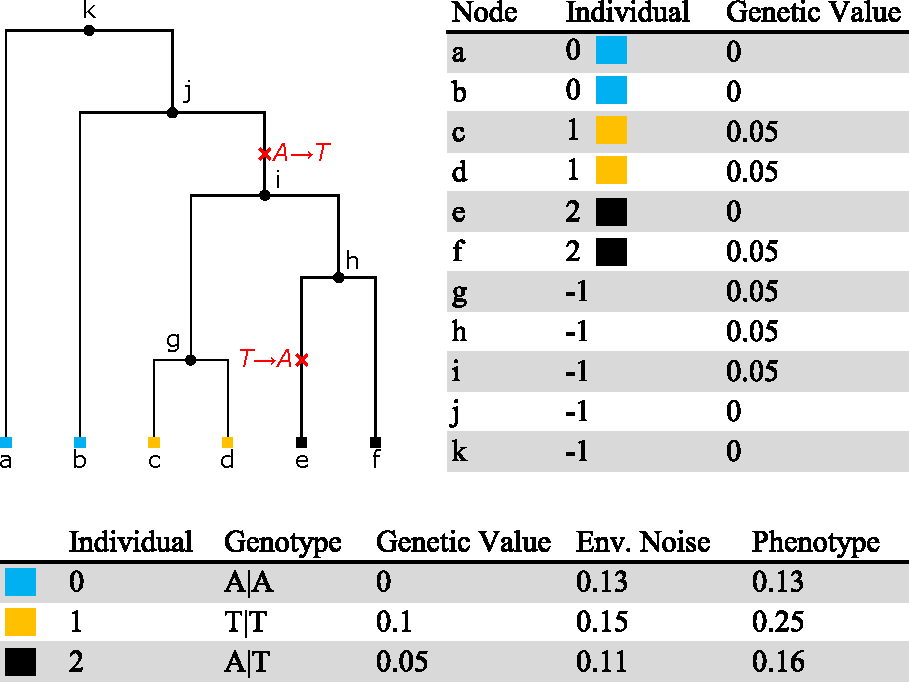
\includegraphics[width=240pt]{figures/tree-illustration.pdf}
\caption{Example simulation of a phenotype at a site with ancestral state A and
two mutations. In this diploid example each of the three individuals
is associated with two nodes (i.e., the individual with ID 0 corresponds
to nodes \textsf{a} and \textsf{b}). Internal nodes in the tree are associated
with the null individual, $-1$. Here, the trait's causal allele is T
with an effect size $\beta=0.05$. Each node in the tree has an associated
genetic value, and the overall genetic value for an individual is the
sum of the genetic values of their corresponding nodes. 
The final phenotype
for each individual is the sum of the genetic value and
simulated environmental noise.
\label{fig:tree-illustration}}
\end{figure}

\subsection{Model}
Phenotypes are simulated in \texttt{tstrait} following standard
GWAS models~\citep{uffelmann2021}, adapted to the ARG context.
Each trait is associated with one or more causal sites
(positions on the genome), and at each causal site there is a causal allele
(i.e.\ a particular nucleotide) associated with an effect size $\beta$.
For each causal site, an effect size is drawn from a distribution
and optionally multiplied by $\left(2p(1-p)\right)^{\alpha/2}$,
where $p$ is the frequency of the causal allele and $\alpha$
is a parameter describing the strength of
frequency dependence~\citep{speed2012}.
At a particular causal site, every node in the local tree that inherits
the causal allele at that site is said to have a ``genetic value'' of $\beta$.
% NOTE removing this for space - it keeps this section on one page.
% Because we are reasoning
% about the inheritance of alleles at a site on the genome,
% we can consider just the local tree at that site and
% the network structure of the ARG is not important~\citep{wong2023general}.

In Fig.~\ref{fig:tree-illustration} we show an example
tree for three individuals.
Because these individuals are diploids, each is associated
with two nodes in the tree (highlighted by colour).
Ancestral nodes are not associated with individuals here,
but in general an ARG may be embedded in a multigenerational
pedigree, where some internal nodes would be associated
with individuals.
In the example of
Fig.~\ref{fig:tree-illustration}, T is chosen as the causal
allele with $\beta=0.05$, 
so all nodes descending from \textsf{i}
have genetic value $0.05$, except \textsf{e} which
has zero because of the back-mutation to A.
Following the standard practise in GWAS~\citep{uffelmann2021},
we assume the additive model such that the overall
genetic value of an individual is the sum of its
nodes' genetic values.
Given these per-individual genetic values, the final phenotype
is then generated by adding some environmental noise.
This noise is simulated from a normal distribution with mean zero
and variance of $V_G(1-h^2)/{h^2}$,
where $V_G$ is the variance of the individual genetic values
and $h^2$ is the narrow-sense heritability provided as input by the user.

\subsection{Interface}
\texttt{Tstrait} is a Python library, building on the \texttt{tskit}
ARG toolkit~\citep{ralph2020,wong2023general} and the rich
Python data-science ecosystem~\citep{numpy}.
Simulating a phenotype for an ARG with default parameter
values requires only a few lines of code:
% NOTE this listing assumes num_causal has been moved, or removed.
% We need to check whether this actually works in the final version.
\begin{lstlisting}[language=Python,aboveskip=1em,belowskip=1em]
import tstrait as tst
model = tst.trait_model('normal', mean=0, var=1)
result = tst.sim_phenotype(arg, model)
\end{lstlisting}
We first create \texttt{model}, which represents the distribution
from which effect sizes are drawn. Five commonly used
univariate distributions are supported, along with the
multivariate normal distribution to model pleiotropic traits.
Given this model, we can then simulate phenotypes for the individuals
in an ARG (as a  \texttt{tskit TreeSequence}) using the
\texttt{sim\_phenotype} function.
The user can either specify a number of causal sites to be chosen randomly
along the genome (one, by default), or can directly provide the causal
sites as input. Combined with the detailed information about
mutations recorded in a \texttt{tskit} ARG, explicitly specifying causal
sites allows us to model many different types of trait, for example
those associated with mutations arising in a particular population
or time interval.
The return value \texttt{result} is an object encapsulating
two Pandas dataframes~\citep{mckinney2010data}: one describing the simulated
effect sizes and the other describing the genetic values,
environmental noise and phenotypes for each individual.
The simulation results can then be efficiently and conveniently
processed using familiar Python data science tools.

As well as this convenient single-function interface,
\texttt{tstrait} provides modular building blocks for power-users
and to facilitate integration with other tools that generate
traits on an ARG. The \texttt{sim\_trait} function
simulates effect sizes for an input ARG, and returns a data frame
describing the causal sites, alleles and effect sizes.
This dataframe can then be passed to the \texttt{genetic\_values}
function, which calculates the genetic values for each
node, and accumulates them by individual
(Fig~\ref{fig:tree-illustration}). Finally, the \texttt{sim\_env}
function takes these per-individual genetic values
and adds some simulated environmental noise to produce the final
phenotypes.

A major benefit of this modular architecture is the flexibility it offers
users. Because the causal sites and effect sizes are specified in a
simple tabular format, users can easily develop their own approach
to simulating these values. Alternatively, other simulators
such as SLiM~\citep{haller2023} that generate effect sizes and
causal mutations during the progress of a forwards-time simulation
could output these
values to a CSV or similar file. The modular architecture  and simple
input data formats are specifically intended to facilitate such
interoperability.

\subsection{Implementation and validation}
\texttt{Tstrait} is written entirely in Python. Numerical operations
are either peformed using standard array-oriented
approaches~\citep{numpy} or accelerated
using the \texttt{numba} JIT compiler~\citep{numba}.
The \texttt{tstrait} codebase includes an extensive suite of unit tests,
which are automatically run as part of the development process. The
output of \texttt{tstrait} has been extensively validated against
theoretical expectations, as well as the output
of \texttt{AlphaSimR}~\citep{gaynor2021} and
\texttt{simplePHENOTYPES}~\citep{fernandes2020}.

\subsection{Performance}
\texttt{Tstrait} is very efficient, and can be applied to datasets at the
largest scales on standard computers.
Supplementary Fig~\ref{fig:time} shows how trait simulation time scales
with number of individuals on human-like coalescent simulations
generated using~\texttt{stdpopsim}~\citep{adrion2020}.
For each ARG, we simulate a trait with 1000 causal sites
and report the mean CPU (Intel(R) Core(TM) i9-11900H)
time over 10 independent replicates.
To emphasise scalability, we also
% TODO check that the numbers align here, we may need to be 
% less specific to avoid confusing readers or having to
% explain technical details.
applied \texttt{tstrait} to the simulations of 2.7 million
French-Canadians discussed in the introduction.
% tstrait simulates phenotypes for 2.7 million individuals in the French Canadian dataset, as ancestors are denoted as individuals in the dataset.
% TODO redo this for 100 causal sites @daiki.
It took 80.69 seconds to simulate a trait with 100 causal sites.
% Is this worth the space? We should cite 1KG project also really.
Finally, to demonstrate that \texttt{tstrait} can also be applied
to ARGs inferred from real data, we simulated a trait with 100 causal
sites for an ARG estimated from 1000 Genomes project
data~\citep{kelleher2019} which has 2,504 samples
and 1,685,401 variant sites. This took 5.40 seconds.
Memory requirements for \texttt{tstrait} are modest: all of the
above experiments were performed on a laptop computer with 16GB of RAM.

\section{Conclusion}
There is substantial interest in using inferred ARGs to improve
association testing
methods~\citep{zhang2023,link2023tree,nowbandegani2023extremely},
and there is a pressing need for a well-tested, efficient
and user-friendly means of simulating phenotypes on ARGs.
Highly realistic simulations conditioned on large
pedigrees~\citep{anderson2023} provide an exciting opportunity
to test the effects of intricate population structure on
GWAS, and we hope that \texttt{tstrait} will facilitate these
investigations. \texttt{Tstrait}'s modular architecture
and flexible specification of causal sites
should provide the opportunity to explore new avenues of research,
and an extensible platform for future development.

\section{Competing interests}
No competing interest is declared.

\section{Acknowledgments}
We are grateful to Gregor Gorjanc, Ben Haller, Ben Jeffery and
others in the tskit community for helpful discussions and feedback.

\section{Funding}
DT is supported by the Oxford Kobe Scholarship from the University of Oxford
and the Euretta J. Kellett Fellowship from Columbia University.
JK acknowledges support from the Robertson Foundation,
NIH (research grants HG011395 and HG012473) and
EPSRC (research grant EP/X024881/1).


%USE THE BELOW OPTIONS IN CASE YOU NEED AUTHOR YEAR FORMAT.
\bibliographystyle{abbrvnat}
\bibliography{paper}

\clearpage

\renewcommand\thefigure{S\arabic{figure}}
\setcounter{figure}{0}
\renewcommand\thetable{S\arabic{table}}
\setcounter{table}{0}
\section{Supplementary Figures}

\begin{figure*}[t]%
\centering
% FIXME get the sizes right here and in the notebook where we're generating
% the figure so we don't have to scale here.
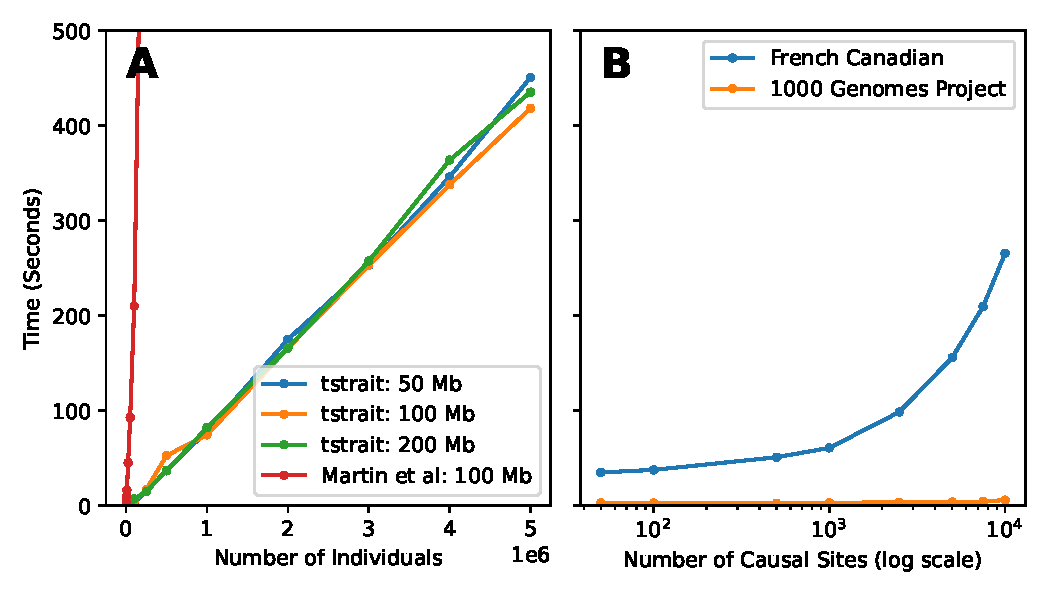
\includegraphics[width=213pt]{figures/time-scaling.pdf}
\caption{\textbf{Time taken to simulate quantitative traits.} Each point
represents the mean time for 10 independent runs under different random seeds.
The times reported are the total CPU time required to simulate quantitative
traits on an Intel(R) Core(TM) i9-11900H CPU and 16 GB of RAM. The trait model
is a normal distribution with $\mu=0$, $\sigma^2=1$, $h^2=0.3$, and
$\alpha=-1$. (A) CPU time with increasing number of individuals
based on ARGs simulated using \texttt{stdpopsim} with the HomSap
demographic mode. For each replicate we simulate
one quantitative trait with 1000 causal sites.
(B) CPU time with increasing number of causal sites on two large ARGs.
\texttt{tstrait} is used to simulate quantitative traits from
the simulated French Canadian dataset \citep{anderson2023} and the inferred
tree sequence dataset of the 1000 Genomes Project \citep{kelleher2019} with
varying number of causal sites. The French Canadian dataset is downloaded from
\url{https://zenodo.org/record/6839683}, and the inferred ARG from the 1000
Genomes Project is downloaded from \url{https://zenodo.org/record/3051855}.
Chromosome 9 is selected for both datasets.}\label{fig:time}
\end{figure*}

\begin{figure*}[t]%
\centering
% FIXME get the sizes right here and in the notebook where we're generating
% the figure so we don't have to scale here.
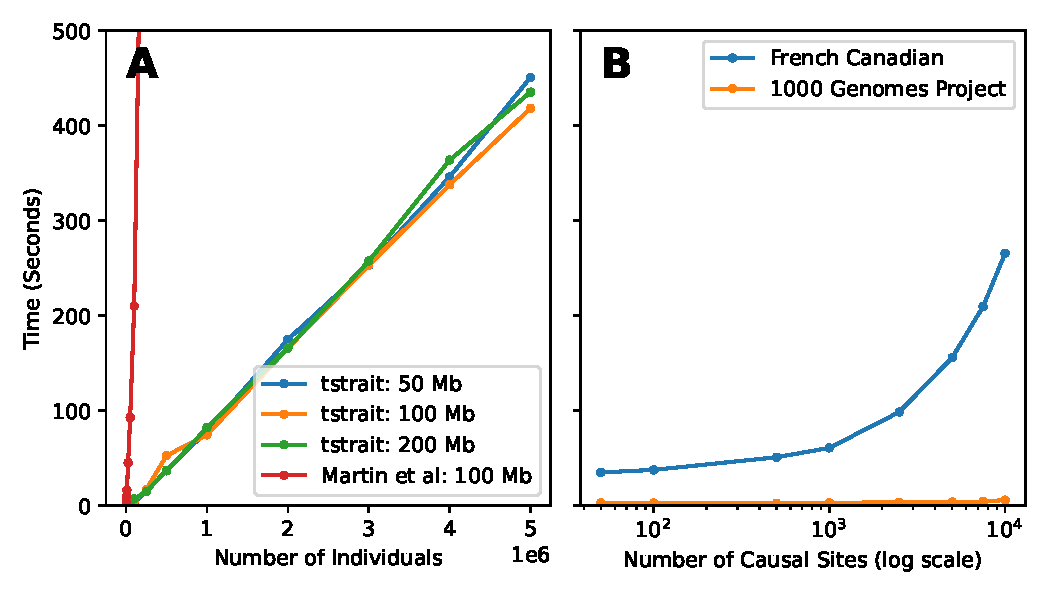
\includegraphics[width=213pt]{figures/time-scaling.pdf}
\caption{\textbf{Time taken to simulate quantitative traits.} Each point
represents the mean time for 10 independent runs under different random seeds with 95\% confidence intervals plotted.
The times reported are the total CPU time required to simulate quantitative
traits on an Intel(R) Core(TM) i9-11900H CPU and 16 GB of RAM. The trait model
is a normal distribution with $\mu=0$, $\sigma^2=1$, $h^2=0.3$, and
$\alpha=0$. \texttt{tstrait} is used to simulate quantitative traits from ARGs simulated using \texttt{stdpopsim} with the HomSap demographic mode. For each replicate we simulate one quantitative trait with 1000 causal sites. We have compared \texttt{tstrait} against the quantitative trait simulation framework that is based on \texttt{tskit} functionalities. The comparison codes are adapted from \citep{martin2017}, and they are modified based on functionalities offered in \texttt{tskit} version 0.5.6 to speed up the computational efficiency.}\label{fig:time}
\end{figure*}
\end{document}
